\documentclass[11pt,]{article}
\usepackage{lmodern}
\usepackage{amssymb,amsmath}
\usepackage{ifxetex,ifluatex}
\usepackage{fixltx2e} % provides \textsubscript
\ifnum 0\ifxetex 1\fi\ifluatex 1\fi=0 % if pdftex
  \usepackage[T1]{fontenc}
  \usepackage[utf8]{inputenc}
\else % if luatex or xelatex
  \ifxetex
    \usepackage{mathspec}
  \else
    \usepackage{fontspec}
  \fi
  \defaultfontfeatures{Ligatures=TeX,Scale=MatchLowercase}
\fi
% use upquote if available, for straight quotes in verbatim environments
\IfFileExists{upquote.sty}{\usepackage{upquote}}{}
% use microtype if available
\IfFileExists{microtype.sty}{%
\usepackage{microtype}
\UseMicrotypeSet[protrusion]{basicmath} % disable protrusion for tt fonts
}{}
\usepackage[left=2cm,right=2cm,top=2cm,bottom=2cm]{geometry}
\usepackage{hyperref}
\hypersetup{unicode=true,
            pdfborder={0 0 0},
            breaklinks=true}
\urlstyle{same}  % don't use monospace font for urls
\usepackage{color}
\usepackage{fancyvrb}
\newcommand{\VerbBar}{|}
\newcommand{\VERB}{\Verb[commandchars=\\\{\}]}
\DefineVerbatimEnvironment{Highlighting}{Verbatim}{commandchars=\\\{\}}
% Add ',fontsize=\small' for more characters per line
\usepackage{framed}
\definecolor{shadecolor}{RGB}{248,248,248}
\newenvironment{Shaded}{\begin{snugshade}}{\end{snugshade}}
\newcommand{\AlertTok}[1]{\textcolor[rgb]{0.94,0.16,0.16}{#1}}
\newcommand{\AnnotationTok}[1]{\textcolor[rgb]{0.56,0.35,0.01}{\textbf{\textit{#1}}}}
\newcommand{\AttributeTok}[1]{\textcolor[rgb]{0.77,0.63,0.00}{#1}}
\newcommand{\BaseNTok}[1]{\textcolor[rgb]{0.00,0.00,0.81}{#1}}
\newcommand{\BuiltInTok}[1]{#1}
\newcommand{\CharTok}[1]{\textcolor[rgb]{0.31,0.60,0.02}{#1}}
\newcommand{\CommentTok}[1]{\textcolor[rgb]{0.56,0.35,0.01}{\textit{#1}}}
\newcommand{\CommentVarTok}[1]{\textcolor[rgb]{0.56,0.35,0.01}{\textbf{\textit{#1}}}}
\newcommand{\ConstantTok}[1]{\textcolor[rgb]{0.00,0.00,0.00}{#1}}
\newcommand{\ControlFlowTok}[1]{\textcolor[rgb]{0.13,0.29,0.53}{\textbf{#1}}}
\newcommand{\DataTypeTok}[1]{\textcolor[rgb]{0.13,0.29,0.53}{#1}}
\newcommand{\DecValTok}[1]{\textcolor[rgb]{0.00,0.00,0.81}{#1}}
\newcommand{\DocumentationTok}[1]{\textcolor[rgb]{0.56,0.35,0.01}{\textbf{\textit{#1}}}}
\newcommand{\ErrorTok}[1]{\textcolor[rgb]{0.64,0.00,0.00}{\textbf{#1}}}
\newcommand{\ExtensionTok}[1]{#1}
\newcommand{\FloatTok}[1]{\textcolor[rgb]{0.00,0.00,0.81}{#1}}
\newcommand{\FunctionTok}[1]{\textcolor[rgb]{0.00,0.00,0.00}{#1}}
\newcommand{\ImportTok}[1]{#1}
\newcommand{\InformationTok}[1]{\textcolor[rgb]{0.56,0.35,0.01}{\textbf{\textit{#1}}}}
\newcommand{\KeywordTok}[1]{\textcolor[rgb]{0.13,0.29,0.53}{\textbf{#1}}}
\newcommand{\NormalTok}[1]{#1}
\newcommand{\OperatorTok}[1]{\textcolor[rgb]{0.81,0.36,0.00}{\textbf{#1}}}
\newcommand{\OtherTok}[1]{\textcolor[rgb]{0.56,0.35,0.01}{#1}}
\newcommand{\PreprocessorTok}[1]{\textcolor[rgb]{0.56,0.35,0.01}{\textit{#1}}}
\newcommand{\RegionMarkerTok}[1]{#1}
\newcommand{\SpecialCharTok}[1]{\textcolor[rgb]{0.00,0.00,0.00}{#1}}
\newcommand{\SpecialStringTok}[1]{\textcolor[rgb]{0.31,0.60,0.02}{#1}}
\newcommand{\StringTok}[1]{\textcolor[rgb]{0.31,0.60,0.02}{#1}}
\newcommand{\VariableTok}[1]{\textcolor[rgb]{0.00,0.00,0.00}{#1}}
\newcommand{\VerbatimStringTok}[1]{\textcolor[rgb]{0.31,0.60,0.02}{#1}}
\newcommand{\WarningTok}[1]{\textcolor[rgb]{0.56,0.35,0.01}{\textbf{\textit{#1}}}}
\usepackage{graphicx,grffile}
\makeatletter
\def\maxwidth{\ifdim\Gin@nat@width>\linewidth\linewidth\else\Gin@nat@width\fi}
\def\maxheight{\ifdim\Gin@nat@height>\textheight\textheight\else\Gin@nat@height\fi}
\makeatother
% Scale images if necessary, so that they will not overflow the page
% margins by default, and it is still possible to overwrite the defaults
% using explicit options in \includegraphics[width, height, ...]{}
\setkeys{Gin}{width=\maxwidth,height=\maxheight,keepaspectratio}
\IfFileExists{parskip.sty}{%
\usepackage{parskip}
}{% else
\setlength{\parindent}{0pt}
\setlength{\parskip}{6pt plus 2pt minus 1pt}
}
\setlength{\emergencystretch}{3em}  % prevent overfull lines
\providecommand{\tightlist}{%
  \setlength{\itemsep}{0pt}\setlength{\parskip}{0pt}}
\setcounter{secnumdepth}{0}
% Redefines (sub)paragraphs to behave more like sections
\ifx\paragraph\undefined\else
\let\oldparagraph\paragraph
\renewcommand{\paragraph}[1]{\oldparagraph{#1}\mbox{}}
\fi
\ifx\subparagraph\undefined\else
\let\oldsubparagraph\subparagraph
\renewcommand{\subparagraph}[1]{\oldsubparagraph{#1}\mbox{}}
\fi

%%% Use protect on footnotes to avoid problems with footnotes in titles
\let\rmarkdownfootnote\footnote%
\def\footnote{\protect\rmarkdownfootnote}

%%% Change title format to be more compact
\usepackage{titling}

% Create subtitle command for use in maketitle
\newcommand{\subtitle}[1]{
  \posttitle{
    \begin{center}\large#1\end{center}
    }
}

\setlength{\droptitle}{-2em}

  \title{}
    \pretitle{\vspace{\droptitle}}
  \posttitle{}
    \author{}
    \preauthor{}\postauthor{}
    \date{}
    \predate{}\postdate{}
  
\usepackage[utf8]{inputenc}
\usepackage[T1]{fontenc}
\usepackage[spanish]{babel}
\usepackage{amsmath}
\usepackage{amsfonts}
\usepackage{amssymb}
%\usepackage{graphicx}
\usepackage{lmodern}
\usepackage{xspace}
\usepackage{multicol}
\usepackage{hyperref}
\usepackage{float}
\usepackage{hyperref}
\usepackage{color}

\newcommand{\azul}[1]{\textcolor{MaterialBlue900}{#1}}
\usepackage{array}

\hypersetup{colorlinks=true,   linkcolor=MaterialBlue900}
%\usepackage[colorlinks=true, linkcolor=black, urlcolor=blue, pdfborder={0 0 0}]{hyperref}
%\usepackage[left=2cm,right=2cm,top=2cm,bottom=2cm]{geometry}
\setlength{\parindent}{0in}
\spanishdecimal{.}

\newcommand{\X}{\mathbb{X}}
\newcommand{\x}{\mathbf{x}}
\newcommand{\Y}{\mathbf{Y}}
\newcommand{\y}{\mathbf{y}}
\newcommand{\xbarn}{\bar{x}_n}
\newcommand{\ybarn}{\bar{y}_n}
\newcommand{\paren}[1]{\left( #1 \right)}
\newcommand{\llaves}[1]{\left\lbrace #1 \right\rbrace}
\newcommand{\barra}{\,\vert\,}
\newcommand{\mP}{\mathbb{P}}
\newcommand{\mE}{\mathbb{E}}
\newcommand{\mI}{\mathbf{I}}
\newcommand{\mJ}{\mathbf{J}}
\newcommand{\mX}{\mathbf{X}}
\newcommand{\mS}{\mathbf{S}}
\newcommand{\mA}{\mathbf{A}}
\newcommand{\unos}{\boldsymbol{1}}
\newcommand{\xbarnv}{\bar{\mathbf{x}}_n}
\newcommand{\abs}[1]{\left\vert #1 \right\vert}
\newcommand{\muv}{\boldsymbol{\mu}}
\newcommand{\mcov}{\boldsymbol{\Sigma}}
\newcommand{\vbet}{\boldsymbol{\beta}}
\newcommand{\veps}{\boldsymbol{\epsilon}}
\newcommand{\mC}{\mathbf{C}}
\newcommand{\ceros}{\boldsymbol{0}}
\newcommand{\mH}{\mathbf{H}}
\newcommand{\ve}{\mathbf{e}}
\newcommand{\avec}{\mathbf{a}}
\newcommand{\res}{\textbf{RESPUESTA}\\}
\newcommand{\rojo}[1]{\textcolor{MaterialRed900}{#1}}

\newcommand{\defi}[3]{\textbf{Definición:#3}}
\newcommand{\fin}{$\blacksquare.$}
\newcommand{\finf}{\blacksquare.}

\begin{document}

\begin{enumerate}
\def\labelenumi{\arabic{enumi}.}
\setcounter{enumi}{3}
\tightlist
\item
  Para el siguiente ejercicio es necesario el programa \textsc{R}.
\end{enumerate}

\begin{enumerate}
\def\labelenumi{\alph{enumi}.}
\tightlist
\item
  Escriba un programa en \textsc{R} que reproduzca las gráficas de las
  funciones de distribución acumulada y de masa de la distribución
  uniforme que aparecen en las notas del curso. Las gráficas deben verse
  similares a las figuras de la Figura 1.
\end{enumerate}

\begin{figure}
\begin{center}
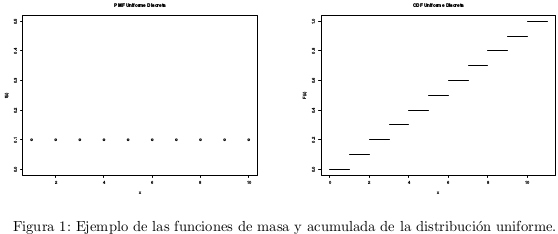
\includegraphics[scale=1]{ejercicio_4-graficas.png}
\end{center}
\end{figure}

\res

Cargamos los paquetes a ocupar:

\begin{Shaded}
\begin{Highlighting}[]
\KeywordTok{library}\NormalTok{(tidyverse)}
\KeywordTok{library}\NormalTok{(gridExtra)}
\end{Highlighting}
\end{Shaded}

Definimos una función que gráfique la función de probabilidad y la
función de probabilidad acumulada para una \(U(0,n)\):

\begin{Shaded}
\begin{Highlighting}[]
\NormalTok{grafica_pdf_and_cdf_uniforme <-}\StringTok{ }\ControlFlowTok{function}\NormalTok{(n)\{ }\CommentTok{# La función tiene como parametro n.}
\NormalTok{    data_uniforme <-}\StringTok{ }\KeywordTok{data_frame}\NormalTok{(}\DataTypeTok{x=}\KeywordTok{seq}\NormalTok{(}\DecValTok{1}\OperatorTok{:}\NormalTok{n)) }\OperatorTok\StringTok{ }
\StringTok{      }\KeywordTok{mutate}\NormalTok{(}\StringTok{"f_x"}\NormalTok{=}\DecValTok{1}\OperatorTok{/}\NormalTok{n, }\CommentTok{# Definimos las probabilidades.}
             \StringTok{"F_x"}\NormalTok{=}\StringTok{ }\KeywordTok{cumsum}\NormalTok{(f_x)) }\CommentTok{# Definimos las probabilidades acumaladas.}
\NormalTok{    data_uniforme[n}\OperatorTok{+}\DecValTok{1}\NormalTok{,]<-}\KeywordTok{c}\NormalTok{(}\DecValTok{0}\NormalTok{,}\OtherTok{NaN}\NormalTok{,}\DecValTok{0}\NormalTok{) }\CommentTok{# Agregamos el valor inicial}
    
\NormalTok{    cdf <-}\StringTok{ }\KeywordTok{ggplot}\NormalTok{(}\DataTypeTok{data=}\NormalTok{data_uniforme)}\OperatorTok{+}\StringTok{ }\CommentTok{# CDF}
\StringTok{      }\KeywordTok{geom_segment}\NormalTok{(}\KeywordTok{aes}\NormalTok{(}\DataTypeTok{x=}\NormalTok{x, }\DataTypeTok{xend=}\NormalTok{x}\OperatorTok{+}\DecValTok{1}\NormalTok{, }\DataTypeTok{y=}\NormalTok{F_x, }\DataTypeTok{yend=}\NormalTok{F_x))}\OperatorTok{+}
\StringTok{      }\KeywordTok{scale_x_discrete}\NormalTok{(}\DataTypeTok{limits=}\KeywordTok{seq}\NormalTok{(}\DecValTok{0}\NormalTok{,n,}\DecValTok{1}\NormalTok{))}\OperatorTok{+}
\StringTok{      }\KeywordTok{labs}\NormalTok{(}\DataTypeTok{y=}\StringTok{"F(x)"}\NormalTok{,}\DataTypeTok{title=}\StringTok{"CDF Unifrome Discreta"}\NormalTok{ )}\OperatorTok{+}\CommentTok{# Graficamos los segementos}
\StringTok{      }\KeywordTok{ylim}\NormalTok{(}\DecValTok{0}\NormalTok{,}\DecValTok{1}\NormalTok{) }\CommentTok{# Limites del eje "y".}
\NormalTok{    pdf <-}\StringTok{ }\KeywordTok{ggplot}\NormalTok{(}\DataTypeTok{data=}\NormalTok{data_uniforme)}\OperatorTok{+}\StringTok{ }\CommentTok{# PDF}
\StringTok{      }\KeywordTok{geom_point}\NormalTok{(}\KeywordTok{aes}\NormalTok{(x,f_x))}\OperatorTok{+}
\StringTok{      }\KeywordTok{geom_segment}\NormalTok{(}\KeywordTok{aes}\NormalTok{(}\DataTypeTok{x=}\NormalTok{x, }\DataTypeTok{xend=}\NormalTok{x, }\DataTypeTok{y=}\DecValTok{0}\NormalTok{, }\DataTypeTok{yend=}\NormalTok{f_x))}\OperatorTok{+}\StringTok{ }\CommentTok{# Graficamos los segementos.}
\StringTok{      }\KeywordTok{scale_x_discrete}\NormalTok{(}\DataTypeTok{limits=}\KeywordTok{seq}\NormalTok{(}\DecValTok{0}\NormalTok{,n,}\DecValTok{1}\NormalTok{))}\OperatorTok{+}
\StringTok{      }\KeywordTok{ylim}\NormalTok{(}\DecValTok{0}\NormalTok{,}\DecValTok{1}\OperatorTok{/}\NormalTok{(n}\DecValTok{-1}\NormalTok{))}\OperatorTok{+}\StringTok{ }\CommentTok{# Límites del eje "y".}
\StringTok{      }\KeywordTok{labs}\NormalTok{(}\DataTypeTok{x=}\StringTok{"x"}\NormalTok{, }\DataTypeTok{y=}\StringTok{"f(x)"}\NormalTok{,}\DataTypeTok{title =} \StringTok{"PDF Unifrome Discreta"}\NormalTok{)}
  \KeywordTok{grid.arrange}\NormalTok{(pdf, cdf, }\DataTypeTok{ncol=}\DecValTok{2}\NormalTok{) }\CommentTok{# Ponemos las gráficas juntas.}
\NormalTok{  \}}
\end{Highlighting}
\end{Shaded}

Mostramos las distribuciones \(U(0,5)\):

\begin{Shaded}
\begin{Highlighting}[]
\KeywordTok{grafica_pdf_and_cdf_uniforme}\NormalTok{(}\DecValTok{5}\NormalTok{) }
\end{Highlighting}
\end{Shaded}

\begin{center}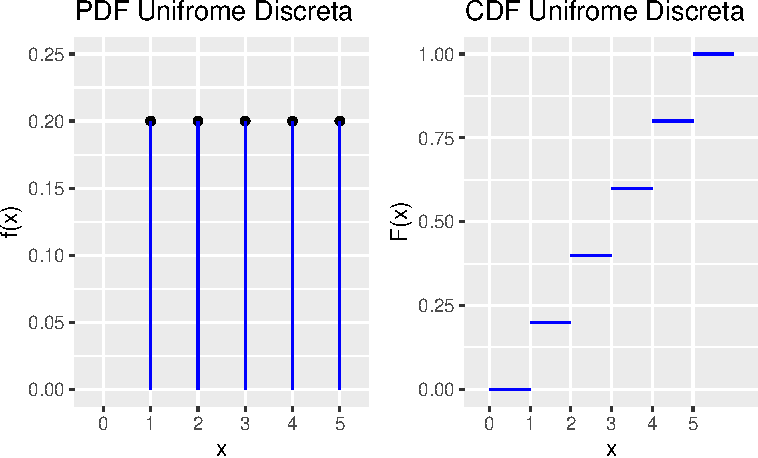
\includegraphics{Tarea_1_files/figure-latex/unnamed-chunk-3-1} \end{center}

\begin{enumerate}
\def\labelenumi{\alph{enumi}.}
\setcounter{enumi}{1}
\item
  Lea en la documentación de \textsc{R}, o en cualquier otra fuente de
  información confiable, la explicación de la función sample(x, size,
  replace=FALSE, prob=NULL). (No es necesario entregar algo para este
  ejercicio).
\item
  Usando la función sample simule una muestra de tamaño 10 000 de la
  distribución U (1, . . . , 10). Fijando la semilla en 13
  (set.seed(13)), muestre los resultados de la simulación en una tabla
  de frecuencia y calcule la media y la varianza. Sugerencia: Use la
  función table.
\end{enumerate}

\res

\begin{Shaded}
\begin{Highlighting}[]
\KeywordTok{set.seed}\NormalTok{(}\DecValTok{13}\NormalTok{) }\CommentTok{# fijamos la semilla.}
\NormalTok{muestra <-}\StringTok{ }\KeywordTok{sample}\NormalTok{(}\DecValTok{10}\NormalTok{, }\DecValTok{10000}\NormalTok{, }\DataTypeTok{replace =} \OtherTok{TRUE}\NormalTok{) }\CommentTok{# Muestra aleatoria.}
\KeywordTok{table}\NormalTok{(muestra) }\CommentTok{# Tabla de Frecuencias}
\end{Highlighting}
\end{Shaded}

\begin{verbatim}
## muestra
##    1    2    3    4    5    6    7    8    9   10 
## 1015 1001  962 1013 1020  982  991  926 1069 1021
\end{verbatim}

\begin{Shaded}
\begin{Highlighting}[]
\KeywordTok{mean}\NormalTok{(muestra) }\CommentTok{# Media de la muestra simulada.}
\end{Highlighting}
\end{Shaded}

\begin{verbatim}
## [1] 5.5123
\end{verbatim}

\begin{Shaded}
\begin{Highlighting}[]
\KeywordTok{var}\NormalTok{(muestra) }\CommentTok{# Varianza de la muestra simulada.}
\end{Highlighting}
\end{Shaded}

\begin{verbatim}
## [1] 8.340283
\end{verbatim}

\begin{enumerate}
\def\labelenumi{\alph{enumi}.}
\setcounter{enumi}{3}
\tightlist
\item
  Grafique las frecuencias de la simulación anterior.
\end{enumerate}

\begin{Shaded}
\begin{Highlighting}[]
\KeywordTok{ggplot}\NormalTok{(}\DataTypeTok{data=}\KeywordTok{data.frame}\NormalTok{(}\DataTypeTok{x=}\NormalTok{muestra), }\KeywordTok{aes}\NormalTok{(x))}\OperatorTok{+}
\StringTok{  }\KeywordTok{geom_bar}\NormalTok{(}\DataTypeTok{fill=}\StringTok{"blue"}\NormalTok{)}\OperatorTok{+}
\StringTok{  }\KeywordTok{scale_x_discrete}\NormalTok{(}\DataTypeTok{limits =}\KeywordTok{seq}\NormalTok{(}\DecValTok{1}\NormalTok{,}\DecValTok{10}\NormalTok{,}\DecValTok{1}\NormalTok{))}\OperatorTok{+}
\StringTok{  }\KeywordTok{labs}\NormalTok{(}\DataTypeTok{title=}\StringTok{"Grafica de frecuencias."}\NormalTok{, }\DataTypeTok{y=}\StringTok{"conteos"}\NormalTok{)}
\end{Highlighting}
\end{Shaded}

\begin{center}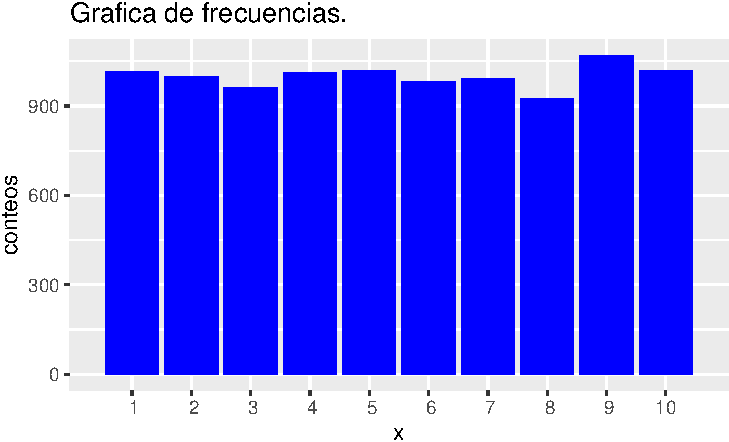
\includegraphics{Tarea_1_files/figure-latex/unnamed-chunk-5-1} \end{center}

\begin{enumerate}
\def\labelenumi{\arabic{enumi}.}
\setcounter{enumi}{4}
\tightlist
\item
  Para el siguiente ejercicio también necesitamos R.
\end{enumerate}

\begin{enumerate}
\def\labelenumi{\alph{enumi}.}
\tightlist
\item
  Usando la función sample, simule 10 lanzamientos de una moneda
  equilibrada y cuente el número de águilas que obtiene. Repita este
  proceso \(10^6\) veces y muestre sus primeros 3 resultados. Grafique
  las frecuencias del número de águilas obtenidas en los \(10^6\)
  experimentos. También grafique las proporciones del número de águilas
  obtenidas.
\end{enumerate}

\res

Consideremos, 1: obtener una aguila, 0: obtener sol.

\begin{Shaded}
\begin{Highlighting}[]
\NormalTok{resultados_modena <-}\StringTok{ }\KeywordTok{c}\NormalTok{(}\DecValTok{0}\NormalTok{,}\DecValTok{1}\NormalTok{)}
\KeywordTok{sum}\NormalTok{(}\KeywordTok{sample}\NormalTok{(resultados_modena, }\DecValTok{10}\NormalTok{, }\DataTypeTok{replace =} \OtherTok{TRUE}\NormalTok{)) }
\end{Highlighting}
\end{Shaded}

\begin{verbatim}
## [1] 6
\end{verbatim}

Ahora repetimos el proceso \(10^6\) veces.

\begin{Shaded}
\begin{Highlighting}[]
\NormalTok{simulacion_moneda_equilibrada <-}\StringTok{ }\KeywordTok{c}\NormalTok{() }\CommentTok{# Inicializamos un vector}
\ControlFlowTok{for}\NormalTok{(i }\ControlFlowTok{in} \DecValTok{1}\OperatorTok{:}\DecValTok{10}\OperatorTok{**}\DecValTok{6}\NormalTok{) \{ }\CommentTok{# Creamos un ciclo para crear las repeticiones.}
\NormalTok{ simulacion_moneda_equilibrada[i] <-}\KeywordTok{sum}\NormalTok{(}\KeywordTok{sample}\NormalTok{(resultados_modena, }\DecValTok{10}\NormalTok{, }\DataTypeTok{replace =} \OtherTok{TRUE}\NormalTok{)) }
\NormalTok{\}}
\CommentTok{# Mostramos los primeros 3 resultados.}
\NormalTok{simulacion_moneda_equilibrada[}\DecValTok{1}\OperatorTok{:}\DecValTok{3}\NormalTok{] }
\end{Highlighting}
\end{Shaded}

\begin{verbatim}
## [1] 3 6 4
\end{verbatim}

Graficamos las frecuencias del número de aguilas obtenidas en cada uno
de los experimentos.

\begin{Shaded}
\begin{Highlighting}[]
\KeywordTok{ggplot}\NormalTok{(}\DataTypeTok{data=}\KeywordTok{data.frame}\NormalTok{(}\DataTypeTok{x=}\NormalTok{simulacion_moneda_equilibrada), }\KeywordTok{aes}\NormalTok{(x))}\OperatorTok{+}
\StringTok{  }\KeywordTok{geom_histogram}\NormalTok{(}\DataTypeTok{bins =} \DecValTok{11}\NormalTok{, }\DataTypeTok{binwidth=}\NormalTok{.}\DecValTok{5}\NormalTok{, }\DataTypeTok{fill=}\StringTok{"blue"}\NormalTok{)}\OperatorTok{+}
\StringTok{  }\KeywordTok{scale_x_discrete}\NormalTok{(}\DataTypeTok{limits=}\KeywordTok{seq}\NormalTok{(}\DecValTok{0}\NormalTok{,}\DecValTok{10}\NormalTok{,}\DecValTok{1}\NormalTok{))}\OperatorTok{+}
\StringTok{  }\KeywordTok{labs}\NormalTok{(}\DataTypeTok{y=}\StringTok{"conteos"}\NormalTok{, }\DataTypeTok{title=}\StringTok{"Grafica de frecuencias del experimiento"}\NormalTok{)}
\end{Highlighting}
\end{Shaded}

\begin{center}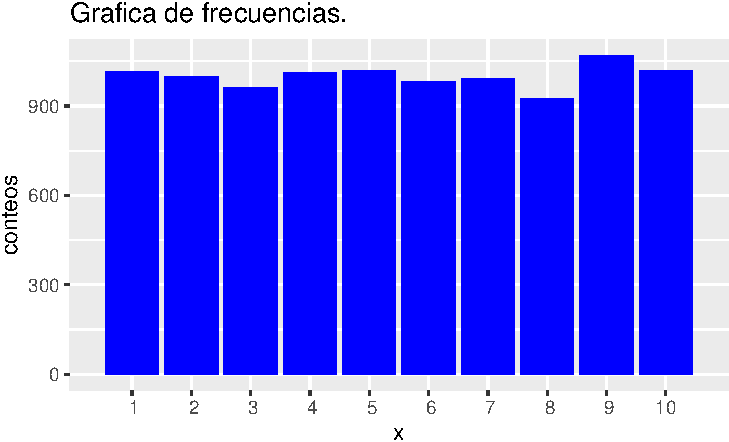
\includegraphics{Tarea_1_files/figure-latex/unnamed-chunk-8-1} \end{center}

\begin{Shaded}
\begin{Highlighting}[]
\KeywordTok{ggplot}\NormalTok{(}\DataTypeTok{data=}\KeywordTok{data.frame}\NormalTok{(}\DataTypeTok{x=}\NormalTok{simulacion_moneda_equilibrada), }\KeywordTok{aes}\NormalTok{(x))}\OperatorTok{+}
\StringTok{  }\KeywordTok{geom_histogram}\NormalTok{(}\DataTypeTok{bins =} \DecValTok{11}\NormalTok{, }\DataTypeTok{binwidth=}\NormalTok{.}\DecValTok{5}\NormalTok{, }\DataTypeTok{fill=}\StringTok{"blue"}\NormalTok{, }\KeywordTok{aes}\NormalTok{(}\DataTypeTok{y=}\KeywordTok{stat}\NormalTok{(count) }\OperatorTok{/}\StringTok{ }\KeywordTok{sum}\NormalTok{(count)))}\OperatorTok{+}
\StringTok{  }\KeywordTok{scale_x_discrete}\NormalTok{(}\DataTypeTok{limits=}\KeywordTok{seq}\NormalTok{(}\DecValTok{0}\NormalTok{,}\DecValTok{10}\NormalTok{,}\DecValTok{1}\NormalTok{))}\OperatorTok{+}
\StringTok{  }\KeywordTok{labs}\NormalTok{(}\DataTypeTok{y=}\StringTok{"conteos"}\NormalTok{, }\DataTypeTok{title=}\StringTok{"Grafica de frecuencias del experimiento"}\NormalTok{)}
\end{Highlighting}
\end{Shaded}

\begin{center}\includegraphics{Tarea_1_files/figure-latex/unnamed-chunk-9-1} \end{center}

\begin{enumerate}
\def\labelenumi{\alph{enumi}.}
\setcounter{enumi}{1}
\tightlist
\item
  Usando la función dbinom grafique la función de masa de una
  distribución B(10, 0.5) sobre la gráfica de las proporciones que hizo
  en el inciso anterior.
\end{enumerate}

\res

\begin{Shaded}
\begin{Highlighting}[]
\NormalTok{binomial<-}\KeywordTok{data.frame}\NormalTok{(}\DataTypeTok{x=}\KeywordTok{seq}\NormalTok{(}\DecValTok{0}\NormalTok{,}\DecValTok{10}\NormalTok{,}\DecValTok{1}\NormalTok{), }\DataTypeTok{y=}\KeywordTok{dbinom}\NormalTok{(}\DataTypeTok{x=}\KeywordTok{seq}\NormalTok{(}\DecValTok{0}\NormalTok{,}\DecValTok{10}\NormalTok{,}\DecValTok{1}\NormalTok{), }\DataTypeTok{size =} \DecValTok{10}\NormalTok{,}\DataTypeTok{prob =} \FloatTok{0.5}\NormalTok{))}
\KeywordTok{ggplot}\NormalTok{(}\DataTypeTok{data=}\KeywordTok{data.frame}\NormalTok{(}\DataTypeTok{x=}\NormalTok{simulacion_moneda_equilibrada), }\KeywordTok{aes}\NormalTok{(x))}\OperatorTok{+}
\StringTok{  }\KeywordTok{geom_histogram}\NormalTok{(}\DataTypeTok{bins =} \DecValTok{11}\NormalTok{, }\DataTypeTok{binwidth=}\NormalTok{.}\DecValTok{5}\NormalTok{, }\DataTypeTok{fill=}\StringTok{"blue"}\NormalTok{, }\KeywordTok{aes}\NormalTok{(}\DataTypeTok{y=}\KeywordTok{stat}\NormalTok{(count)}\OperatorTok{/}\KeywordTok{sum}\NormalTok{(count)))}\OperatorTok{+}
\StringTok{  }\KeywordTok{scale_x_discrete}\NormalTok{(}\DataTypeTok{limits=}\KeywordTok{seq}\NormalTok{(}\DecValTok{0}\NormalTok{,}\DecValTok{10}\NormalTok{,}\DecValTok{1}\NormalTok{))}\OperatorTok{+}
\StringTok{  }\KeywordTok{labs}\NormalTok{(}\DataTypeTok{y=}\StringTok{"proporción", title="}\NormalTok{Grafica de frecuencias del experimiento}\StringTok{")+}
\StringTok{  geom_line(data=binomial, aes(x,y))+}
\StringTok{  geom_point(data=binomial, aes(x,y))}
\end{Highlighting}
\end{Shaded}

\begin{center}\includegraphics{Tarea_1_files/figure-latex/unnamed-chunk-10-1} \end{center}

\begin{enumerate}
\def\labelenumi{\alph{enumi}.}
\setcounter{enumi}{2}
\tightlist
\item
  Repita los dos incisos anteriores para una moneda desequilibrada que
  tiene probabilidad \(p = 0.3\) de obtener un águila cuando se lanza.
  ¿Qué observa?
\end{enumerate}

\res

Primero consideremos una moneda desequilibrado con probabilidad de 0.3
de obtener águila.

\begin{Shaded}
\begin{Highlighting}[]
\NormalTok{lanzamientos_moneda_desequilibrada <-}\StringTok{ }\KeywordTok{c}\NormalTok{(}\KeywordTok{rep}\NormalTok{(}\DecValTok{0}\NormalTok{,}\DecValTok{7}\NormalTok{),}\KeywordTok{rep}\NormalTok{(}\DecValTok{1}\NormalTok{,}\DecValTok{3}\NormalTok{))}
\end{Highlighting}
\end{Shaded}

Simulamos 10 lanzamientos de la6 moneda, y contamos el número de águilas
en la simulación:

\begin{Shaded}
\begin{Highlighting}[]
\KeywordTok{sum}\NormalTok{(}\KeywordTok{sample}\NormalTok{(lanzamientos_moneda_desequilibrada, }\DecValTok{10}\NormalTok{, }\DataTypeTok{replace =} \OtherTok{TRUE}\NormalTok{))}
\end{Highlighting}
\end{Shaded}

\begin{verbatim}
## [1] 2
\end{verbatim}

Ahora realizamos este experimento \(10^6\) veces.

\begin{Shaded}
\begin{Highlighting}[]
\NormalTok{simulacion_monedas_desequilibrada <-}\StringTok{ }\KeywordTok{c}\NormalTok{() }\CommentTok{#inicializamos el vector de resultados. }
\ControlFlowTok{for}\NormalTok{(i }\ControlFlowTok{in} \DecValTok{1}\OperatorTok{:}\DecValTok{10}\OperatorTok{**}\DecValTok{6}\NormalTok{) \{}
\NormalTok{simulacion_monedas_desequilibrada[i] <-}\KeywordTok{sum}\NormalTok{(}\KeywordTok{sample}\NormalTok{(lanzamientos_moneda_desequilibrada, }\DecValTok{10}\NormalTok{, }\DataTypeTok{replace =} \OtherTok{TRUE}\NormalTok{))}
\DecValTok{4}\NormalTok{\}}
\end{Highlighting}
\end{Shaded}

Mostramos los primeros 3 resultados:

\begin{Shaded}
\begin{Highlighting}[]
\NormalTok{simulacion_monedas_desequilibrada[}\DecValTok{1}\OperatorTok{:}\DecValTok{3}\NormalTok{]}
\end{Highlighting}
\end{Shaded}

\begin{verbatim}
## [1] 2 3 4
\end{verbatim}

Graficamos las frecuencias del número de aguilas obtenidas en cada uno
de los experimentos:

\begin{Shaded}
\begin{Highlighting}[]
\KeywordTok{ggplot}\NormalTok{(}\DataTypeTok{data=}\KeywordTok{data.frame}\NormalTok{(}\DataTypeTok{x=}\NormalTok{simulacion_monedas_desequilibrada), }\KeywordTok{aes}\NormalTok{(x))}\OperatorTok{+}
\KeywordTok{geom_histogram}\NormalTok{(}\DataTypeTok{bins =} \DecValTok{11}\NormalTok{, }\DataTypeTok{binwidth=}\NormalTok{.}\DecValTok{5}\NormalTok{, }\DataTypeTok{fill=}\StringTok{"blue"}\NormalTok{)}\OperatorTok{+}
\KeywordTok{scale_x_discrete}\NormalTok{(}\DataTypeTok{limits=}\KeywordTok{seq}\NormalTok{(}\DecValTok{0}\NormalTok{,}\DecValTok{10}\NormalTok{,}\DecValTok{1}\NormalTok{))}\OperatorTok{+}
\KeywordTok{labs}\NormalTok{(}\DataTypeTok{y=}\StringTok{"conteos"}\NormalTok{, }\DataTypeTok{title=}\StringTok{"Grafica de frecuencias del experimiento"}\NormalTok{)}
\end{Highlighting}
\end{Shaded}

\begin{center}\includegraphics{Tarea_1_files/figure-latex/unnamed-chunk-15-1} \end{center}

Graficamos las proporciones del número de águilas obtenidas:

\begin{Shaded}
\begin{Highlighting}[]
\KeywordTok{ggplot}\NormalTok{(}\DataTypeTok{data=}\KeywordTok{data.frame}\NormalTok{(}\DataTypeTok{x=}\NormalTok{simulacion_monedas_desequilibrada), }\KeywordTok{aes}\NormalTok{(x))}\OperatorTok{+}
\KeywordTok{geom_histogram}\NormalTok{(}\DataTypeTok{bins =} \DecValTok{11}\NormalTok{, }\DataTypeTok{binwidth=}\NormalTok{.}\DecValTok{5}\NormalTok{, }\DataTypeTok{fill=}\StringTok{"blue"}\NormalTok{, }\KeywordTok{aes}\NormalTok{(}\DataTypeTok{y=}\KeywordTok{stat}\NormalTok{(count)}\OperatorTok{/}\KeywordTok{sum}\NormalTok{(count)))}\OperatorTok{+}
\KeywordTok{scale_x_discrete}\NormalTok{(}\DataTypeTok{limits=}\KeywordTok{seq}\NormalTok{(}\DecValTok{0}\NormalTok{,}\DecValTok{10}\NormalTok{,}\DecValTok{1}\NormalTok{))}\OperatorTok{+}
\KeywordTok{labs}\NormalTok{(}\DataTypeTok{y=}\StringTok{"conteos"}\NormalTok{, }\DataTypeTok{title=}\StringTok{"Grafica de frecuencias del experimiento"}\NormalTok{)}
\end{Highlighting}
\end{Shaded}

\begin{center}\includegraphics{Tarea_1_files/figure-latex/unnamed-chunk-16-1} \end{center}

Usando la función dbinom graficamos la función de masa de una
distribución \(B(10,0.5)\) sobre la gráfica anterior:

\begin{Shaded}
\begin{Highlighting}[]
\NormalTok{binomial<-}\KeywordTok{data.frame}\NormalTok{(}\DataTypeTok{x=}\KeywordTok{seq}\NormalTok{(}\DecValTok{0}\NormalTok{,}\DecValTok{10}\NormalTok{,}\DecValTok{1}\NormalTok{), }\DataTypeTok{y=}\KeywordTok{dbinom}\NormalTok{(}\DataTypeTok{x=}\KeywordTok{seq}\NormalTok{(}\DecValTok{0}\NormalTok{,}\DecValTok{10}\NormalTok{,}\DecValTok{1}\NormalTok{), }\DataTypeTok{size =} \DecValTok{10}\NormalTok{,}\DataTypeTok{prob =} \FloatTok{0.3}\NormalTok{))}
\KeywordTok{ggplot}\NormalTok{(}\DataTypeTok{data=}\KeywordTok{data.frame}\NormalTok{(}\DataTypeTok{x=}\NormalTok{simulacion_monedas_desequilibrada), }\KeywordTok{aes}\NormalTok{(x))}\OperatorTok{+}
\KeywordTok{geom_histogram}\NormalTok{(}\DataTypeTok{bins =} \DecValTok{11}\NormalTok{, }\DataTypeTok{binwidth=}\NormalTok{.}\DecValTok{5}\NormalTok{, }\DataTypeTok{fill=}\StringTok{"blue"}\NormalTok{, }\KeywordTok{aes}\NormalTok{(}\DataTypeTok{y=}\KeywordTok{stat}\NormalTok{(count)}\OperatorTok{/}\KeywordTok{sum}\NormalTok{(count)))}\OperatorTok{+}
\KeywordTok{scale_x_discrete}\NormalTok{(}\DataTypeTok{limits=}\KeywordTok{seq}\NormalTok{(}\DecValTok{0}\NormalTok{,}\DecValTok{10}\NormalTok{,}\DecValTok{1}\NormalTok{))}\OperatorTok{+}
\KeywordTok{labs}\NormalTok{(}\DataTypeTok{y=}\StringTok{"proporción", title="}\NormalTok{Grafica de frecuencias del experimiento}\StringTok{")+}
\StringTok{geom_line(data=binomial, aes(x,y))+}
\StringTok{geom_point(data=binomial, aes(x,y))}
\end{Highlighting}
\end{Shaded}

\begin{center}\includegraphics{Tarea_1_files/figure-latex/unnamed-chunk-17-1} \end{center}

\begin{enumerate}
\def\labelenumi{\arabic{enumi}.}
\setcounter{enumi}{5}
\tightlist
\item
  Una urna contiene 46 bolas grises y 49 bolas blancas. Usando la
  función sample en R, simule la extracción sin reemplazamiento de 20 de
  estas bolas y cuente el número de bolas grises que obtuvo. Repita este
  proceso \(10^6\) veces y grafique las frecuencias de bolas grises
  obtenidas en cada experimento. ¿Cuál es la probabilidad de que al
  extraer 20 bolas de la urna 5 de ellas sean grises? También grafique
  la proporción de bolas grises obtenidas en los experiementos
  anteriores y sobre esta figura añada la correspondiente función de
  masa de la distristibución Hipergeometrica asociada al experimento
  total.
\end{enumerate}

\res

Sea 1: una bola gris, y 0: una bola blanca.

\begin{Shaded}
\begin{Highlighting}[]
\NormalTok{urna <-}\StringTok{ }\KeywordTok{c}\NormalTok{(}\KeywordTok{rep}\NormalTok{(}\DecValTok{1}\NormalTok{,}\DecValTok{46}\NormalTok{), }\KeywordTok{rep}\NormalTok{(}\DecValTok{0}\NormalTok{,}\DecValTok{49}\NormalTok{)) }\CommentTok{# Creamos la urna con las bolas.}
\KeywordTok{sum}\NormalTok{(}\KeywordTok{sample}\NormalTok{(urna, }\DecValTok{20}\NormalTok{, }\DataTypeTok{replace=}\OtherTok{FALSE}\NormalTok{)) }\CommentTok{# Contamos cuantas bolas grises hay en la muestra.}
\end{Highlighting}
\end{Shaded}

\begin{verbatim}
## [1] 9
\end{verbatim}

\begin{Shaded}
\begin{Highlighting}[]
\NormalTok{simulacion_bolas <-}\StringTok{ }\KeywordTok{c}\NormalTok{() }\CommentTok{#Inicializamos }
\ControlFlowTok{for}\NormalTok{(i }\ControlFlowTok{in} \DecValTok{1}\OperatorTok{:}\DecValTok{10}\OperatorTok{**}\DecValTok{6}\NormalTok{) \{ }\CommentTok{# Repetimos el experimento de extraer una muestra.}
\NormalTok{ simulacion_bolas[i] <-}\KeywordTok{sum}\NormalTok{(}\KeywordTok{sample}\NormalTok{(urna, }\DecValTok{20}\NormalTok{, }\DataTypeTok{replace=}\OtherTok{FALSE}\NormalTok{))}
\NormalTok{\}}
\end{Highlighting}
\end{Shaded}

\begin{Shaded}
\begin{Highlighting}[]
\KeywordTok{ggplot}\NormalTok{(}\DataTypeTok{data=}\KeywordTok{data.frame}\NormalTok{(}\DataTypeTok{x=}\NormalTok{simulacion_bolas), }\KeywordTok{aes}\NormalTok{(x))}\OperatorTok{+}
\StringTok{  }\KeywordTok{geom_histogram}\NormalTok{(}\DataTypeTok{bins =} \DecValTok{19}\NormalTok{, }\DataTypeTok{binwidth=}\NormalTok{.}\DecValTok{5}\NormalTok{, }\DataTypeTok{fill=}\StringTok{"blue"}\NormalTok{)}\OperatorTok{+}
\StringTok{  }\KeywordTok{scale_x_discrete}\NormalTok{(}\DataTypeTok{limits=}\KeywordTok{seq}\NormalTok{(}\DecValTok{0}\NormalTok{,}\DecValTok{20}\NormalTok{,}\DecValTok{1}\NormalTok{))}\OperatorTok{+}
\StringTok{  }\KeywordTok{labs}\NormalTok{(}\DataTypeTok{y=}\StringTok{"conteos"}\NormalTok{, }\DataTypeTok{title=}\StringTok{"Grafica de frecuencias del experimiento"}\NormalTok{)}
\end{Highlighting}
\end{Shaded}

\begin{center}\includegraphics{Tarea_1_files/figure-latex/unnamed-chunk-20-1} \end{center}

Si \(X\) es el número es de bolas grises que se obtienen en la
extracción sin reemplazamiento de 20 bolas de la urna definida en el
problema, entonces podemos decir que \(X\sim Hyper(n=20, M=46, N=95)\).
Por lo tanto, la porbabilidad de que se extraigan 5 bolas grises es:

\[f(x=5)=\frac{{46 \choose 5}{49 \choose 15}}{{95 \choose 20}}=0.01261935. \]

Graficamos la proporción de bolas grises:

\begin{Shaded}
\begin{Highlighting}[]
\NormalTok{hyper<-}\KeywordTok{data.frame}\NormalTok{(}\DataTypeTok{x=}\KeywordTok{seq}\NormalTok{(}\DecValTok{0}\NormalTok{,}\DecValTok{20}\NormalTok{,}\DecValTok{1}\NormalTok{), }\DataTypeTok{y=}\KeywordTok{dhyper}\NormalTok{(}\DataTypeTok{x=}\KeywordTok{seq}\NormalTok{(}\DecValTok{0}\NormalTok{,}\DecValTok{20}\NormalTok{,}\DecValTok{1}\NormalTok{), }\DataTypeTok{m =} \DecValTok{46}\NormalTok{, }\DataTypeTok{n=}\DecValTok{49}\NormalTok{, }\DataTypeTok{k=}\DecValTok{20}\NormalTok{))}
\KeywordTok{ggplot}\NormalTok{(}\DataTypeTok{data=}\KeywordTok{data.frame}\NormalTok{(}\DataTypeTok{x=}\NormalTok{simulacion_bolas), }\KeywordTok{aes}\NormalTok{(x))}\OperatorTok{+}
\StringTok{  }\KeywordTok{geom_histogram}\NormalTok{(}\DataTypeTok{bins =} \DecValTok{21}\NormalTok{, }\DataTypeTok{binwidth=}\NormalTok{.}\DecValTok{5}\NormalTok{, }\DataTypeTok{fill=}\StringTok{"blue"}\NormalTok{, }\KeywordTok{aes}\NormalTok{(}\DataTypeTok{y=}\KeywordTok{stat}\NormalTok{(count)}\OperatorTok{/}\KeywordTok{sum}\NormalTok{(count)))}\OperatorTok{+}
\StringTok{  }\KeywordTok{scale_x_discrete}\NormalTok{(}\DataTypeTok{limits=}\KeywordTok{seq}\NormalTok{(}\DecValTok{0}\NormalTok{,}\DecValTok{20}\NormalTok{,}\DecValTok{1}\NormalTok{))}\OperatorTok{+}
\StringTok{  }\KeywordTok{labs}\NormalTok{(}\DataTypeTok{y=}\StringTok{"proporción", title="}\NormalTok{Grafica de frecuencias del experimiento}\StringTok{")+}
\StringTok{  geom_line(data=hyper, aes(x,y))+}
\StringTok{  geom_point(data=hyper, aes(x,y))}
\end{Highlighting}
\end{Shaded}

\begin{center}\includegraphics{Tarea_1_files/figure-latex/unnamed-chunk-21-1} \end{center}


\end{document}
